\documentclass[14pt,a4paper]{article}
\renewcommand{\baselinestretch}{0.5}
\usepackage{lipsum}
\usepackage[margin=1in,includefoot]{geometry}
	\usepackage{listings}
	\usepackage{verbatim}
	\usepackage{graphicx}
\usepackage{float}


\begin{document}
	\begin{titlepage}
	\begin{center}
	\Huge{\bfseries ASSIGNMENT-5}\\
	[5mm]
	\Large{FINANCIAL MATHEMATICS}\\
	[15cm]
	\end{center}
	
	\begin{flushright}
	Submitted by-\\
	[2mm]	
	\textsc{\Large Debwashis}\\
	[0.1cm]	
	4th year\\
	class Roll: JN-020-038\\
	Department of Applied Mathematics\\
	January 13, 2019\\
	\end{flushright}
	\end{titlepage}
	\noindent Consider the equation for geometric Brownian motion, as used to model the path of an underlying asset: 
\begin{equation}
dS=\mu Sdt+\sigma Sdt
\end{equation}		
where $dX$ is the increment of a Wiener process (drawn from a Normal distribution with mean zero and standard deviation $\sqrt{dt}$); we may then write that
\begin{equation}
dX=\phi \sqrt{dt}
\end{equation}
	where $\phi$ is a random variable drawn from a normalised Normal distribution. Utilising eq(2) and risk neutrally, (1) can be integrated exactly over a timescale $\delta t$ (NOT necessarily small) to yield 
	\begin{equation}
	S(t+\delta t) = S(t) exp((r-\frac{1}{2}\sigma^2)\delta t+\sigma \phi \sqrt{\delta t})
	\end{equation}
	equation (3) then generates a random path. Since $\delta t$ need not be small, in the case of European options, it is possible to generate a (random) value of S at expiry (t=T) in just one step (i.e $\delta t=T$). From this value (say S(T)), the payoff can be easily calculated  (max(S(T)X,0) in the case of call option). If this payoff is denoted as, $Payoff_i$ (for the $i^th$ simulation), then the value of this payoff at t=0 is 
	\begin{equation}
	C_i(t=0)=Payoff_i{e^{-rT}}=max(S(T)-X,0)e^{-rT}
	\end{equation}
	If N simulations are performed, then we merely average out the $C_i(t=0)$ to yield  an approximation for the value of the call, i.e\\
	\begin{equation}
	C=\frac{\sum_{i=1}^N C_i(t=0)}{N}\\
	\end{equation}
	\\
	[1in]
	\# We have to calculate the value of a European call and put option, with S(t=0)=5, X=5, r=0.04, $\sigma$=0.2, T=0.5 .\\
	\# We have to plot the value of the two options with increasing N (N=1000,2000,.....,50000 or more!).\\
	\# We have to compare the obtained values with the exact values.\\
	\# And we have to determine how accurately the values of our call and put options satisfy the put-call parity relationship with increasing N (N=1000,2000,....,50000 or more). \\
	[1in]
	
\lstset{ 
	language=Matlab,                		
	numbers=left,                  				
	numberstyle=\footnotesize,      			
	stepnumber=1,                   				
	numbersep=5pt,                  		
	showspaces=false,               					
	showstringspaces=false,         		
	breaklines=true,                					
	breakatwhitespace=false,        				
	escapeinside={\%*}{*)}          		
}

\Large{File Name: {\bf callput.m}}\\
    \lstinputlisting[language=Matlab]{callput.m}
\vspace{1in}
\Large{File Name: {\bf cppayoff.m}}\\
\lstinputlisting[language=Matlab]{cppayoff.m}
\vspace{1in}
\Large{File Name: {\bf output.txt}}\\
\verbatiminput{output.txt}


\begin{figure}[H]
\centering
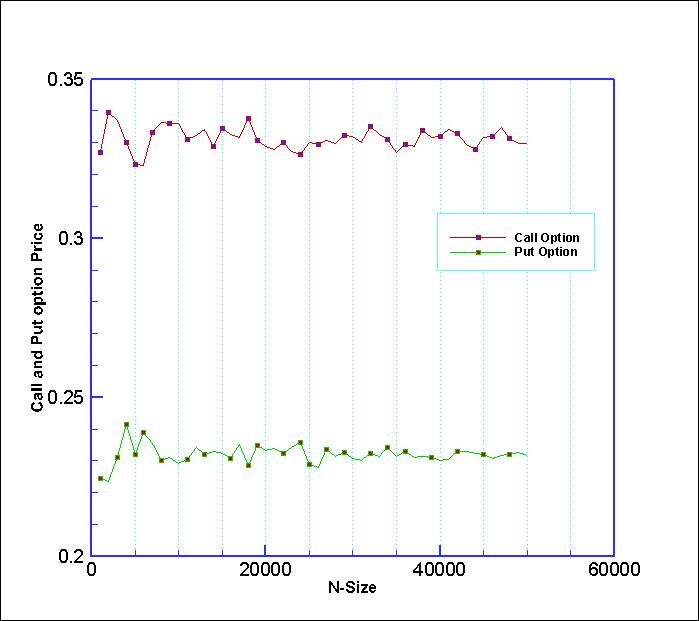
\includegraphics[height=5in]{figure1.jpeg}
\end{figure}
	\end{document}
